\documentclass[]{article}
\usepackage{lmodern}
\usepackage{amssymb,amsmath}
\usepackage{ifxetex,ifluatex}
\usepackage{fixltx2e} % provides \textsubscript
\ifnum 0\ifxetex 1\fi\ifluatex 1\fi=0 % if pdftex
  \usepackage[T1]{fontenc}
  \usepackage[utf8]{inputenc}
\else % if luatex or xelatex
  \ifxetex
    \usepackage{mathspec}
  \else
    \usepackage{fontspec}
  \fi
  \defaultfontfeatures{Ligatures=TeX,Scale=MatchLowercase}
\fi
% use upquote if available, for straight quotes in verbatim environments
\IfFileExists{upquote.sty}{\usepackage{upquote}}{}
% use microtype if available
\IfFileExists{microtype.sty}{%
\usepackage{microtype}
\UseMicrotypeSet[protrusion]{basicmath} % disable protrusion for tt fonts
}{}
\usepackage[margin=1in]{geometry}
\usepackage{hyperref}
\hypersetup{unicode=true,
            pdftitle={Sources of Misperception: Media Choice and the Economic Impact of Legal Immigration},
            pdfauthor={Patrick W. Kraft; Nicholas R. Davis; Taraleigh Davis; Amanda J. Heideman; Jason T. Neumeyer; Shin Young Park},
            pdfborder={0 0 0},
            breaklinks=true}
\urlstyle{same}  % don't use monospace font for urls
\usepackage{color}
\usepackage{fancyvrb}
\newcommand{\VerbBar}{|}
\newcommand{\VERB}{\Verb[commandchars=\\\{\}]}
\DefineVerbatimEnvironment{Highlighting}{Verbatim}{commandchars=\\\{\}}
% Add ',fontsize=\small' for more characters per line
\usepackage{framed}
\definecolor{shadecolor}{RGB}{248,248,248}
\newenvironment{Shaded}{\begin{snugshade}}{\end{snugshade}}
\newcommand{\AlertTok}[1]{\textcolor[rgb]{0.94,0.16,0.16}{#1}}
\newcommand{\AnnotationTok}[1]{\textcolor[rgb]{0.56,0.35,0.01}{\textbf{\textit{#1}}}}
\newcommand{\AttributeTok}[1]{\textcolor[rgb]{0.77,0.63,0.00}{#1}}
\newcommand{\BaseNTok}[1]{\textcolor[rgb]{0.00,0.00,0.81}{#1}}
\newcommand{\BuiltInTok}[1]{#1}
\newcommand{\CharTok}[1]{\textcolor[rgb]{0.31,0.60,0.02}{#1}}
\newcommand{\CommentTok}[1]{\textcolor[rgb]{0.56,0.35,0.01}{\textit{#1}}}
\newcommand{\CommentVarTok}[1]{\textcolor[rgb]{0.56,0.35,0.01}{\textbf{\textit{#1}}}}
\newcommand{\ConstantTok}[1]{\textcolor[rgb]{0.00,0.00,0.00}{#1}}
\newcommand{\ControlFlowTok}[1]{\textcolor[rgb]{0.13,0.29,0.53}{\textbf{#1}}}
\newcommand{\DataTypeTok}[1]{\textcolor[rgb]{0.13,0.29,0.53}{#1}}
\newcommand{\DecValTok}[1]{\textcolor[rgb]{0.00,0.00,0.81}{#1}}
\newcommand{\DocumentationTok}[1]{\textcolor[rgb]{0.56,0.35,0.01}{\textbf{\textit{#1}}}}
\newcommand{\ErrorTok}[1]{\textcolor[rgb]{0.64,0.00,0.00}{\textbf{#1}}}
\newcommand{\ExtensionTok}[1]{#1}
\newcommand{\FloatTok}[1]{\textcolor[rgb]{0.00,0.00,0.81}{#1}}
\newcommand{\FunctionTok}[1]{\textcolor[rgb]{0.00,0.00,0.00}{#1}}
\newcommand{\ImportTok}[1]{#1}
\newcommand{\InformationTok}[1]{\textcolor[rgb]{0.56,0.35,0.01}{\textbf{\textit{#1}}}}
\newcommand{\KeywordTok}[1]{\textcolor[rgb]{0.13,0.29,0.53}{\textbf{#1}}}
\newcommand{\NormalTok}[1]{#1}
\newcommand{\OperatorTok}[1]{\textcolor[rgb]{0.81,0.36,0.00}{\textbf{#1}}}
\newcommand{\OtherTok}[1]{\textcolor[rgb]{0.56,0.35,0.01}{#1}}
\newcommand{\PreprocessorTok}[1]{\textcolor[rgb]{0.56,0.35,0.01}{\textit{#1}}}
\newcommand{\RegionMarkerTok}[1]{#1}
\newcommand{\SpecialCharTok}[1]{\textcolor[rgb]{0.00,0.00,0.00}{#1}}
\newcommand{\SpecialStringTok}[1]{\textcolor[rgb]{0.31,0.60,0.02}{#1}}
\newcommand{\StringTok}[1]{\textcolor[rgb]{0.31,0.60,0.02}{#1}}
\newcommand{\VariableTok}[1]{\textcolor[rgb]{0.00,0.00,0.00}{#1}}
\newcommand{\VerbatimStringTok}[1]{\textcolor[rgb]{0.31,0.60,0.02}{#1}}
\newcommand{\WarningTok}[1]{\textcolor[rgb]{0.56,0.35,0.01}{\textbf{\textit{#1}}}}
\usepackage{graphicx,grffile}
\makeatletter
\def\maxwidth{\ifdim\Gin@nat@width>\linewidth\linewidth\else\Gin@nat@width\fi}
\def\maxheight{\ifdim\Gin@nat@height>\textheight\textheight\else\Gin@nat@height\fi}
\makeatother
% Scale images if necessary, so that they will not overflow the page
% margins by default, and it is still possible to overwrite the defaults
% using explicit options in \includegraphics[width, height, ...]{}
\setkeys{Gin}{width=\maxwidth,height=\maxheight,keepaspectratio}
\IfFileExists{parskip.sty}{%
\usepackage{parskip}
}{% else
\setlength{\parindent}{0pt}
\setlength{\parskip}{6pt plus 2pt minus 1pt}
}
\setlength{\emergencystretch}{3em}  % prevent overfull lines
\providecommand{\tightlist}{%
  \setlength{\itemsep}{0pt}\setlength{\parskip}{0pt}}
\setcounter{secnumdepth}{5}
% Redefines (sub)paragraphs to behave more like sections
\ifx\paragraph\undefined\else
\let\oldparagraph\paragraph
\renewcommand{\paragraph}[1]{\oldparagraph{#1}\mbox{}}
\fi
\ifx\subparagraph\undefined\else
\let\oldsubparagraph\subparagraph
\renewcommand{\subparagraph}[1]{\oldsubparagraph{#1}\mbox{}}
\fi

%%% Use protect on footnotes to avoid problems with footnotes in titles
\let\rmarkdownfootnote\footnote%
\def\footnote{\protect\rmarkdownfootnote}

%%% Change title format to be more compact
\usepackage{titling}

% Create subtitle command for use in maketitle
\providecommand{\subtitle}[1]{
  \posttitle{
    \begin{center}\large#1\end{center}
    }
}

\setlength{\droptitle}{-2em}

  \title{Sources of Misperception: Media Choice and the Economic Impact
of Legal Immigration}
    \pretitle{\vspace{\droptitle}\centering\huge}
  \posttitle{\par}
  \subtitle{Pre-Analysis Plan}
  \author{Patrick W. Kraft \\ Nicholas R. Davis \\ Taraleigh
Davis \\ Amanda J. Heideman \\ Jason T. Neumeyer \\ Shin Young Park}
    \preauthor{\centering\large\emph}
  \postauthor{\par}
      \predate{\centering\large\emph}
  \postdate{\par}
    \date{\today}

\renewcommand{\familydefault}{\sfdefault} \usepackage{float}

\floatplacement{figure}{H}

\begin{document}
\maketitle
\begin{abstract}
Various important issues at the center of today's politics---such as
immigration or climate change---are imbued with citizens'
misperceptions. A growing body of research therefore explores whether
such misperceptions can be mitigated by providing corrective
information. While such corrections have been shown to reduce factual
misperceptions, they appear to have little to no effect on underlying
attitudes. Our study contributes to this active research area by
examining how variations in the source and delivery mode of corrective
information moderate their effectiveness. In our experimental design,
respondents are exposed to a news article about immigration reported by
either Fox News or MSNBC. The main treatment consists of either allowing
free choice of the respective media source or assigning it randomly. Our
outcomes of interest focus on the perceived economic impact of legal
immigration, attitudes towards immigrants, and engagement with the news
article. In order to isolate the effect of delivery mode and messenger,
the news content is held constant across news sources.
\end{abstract}

\hypertarget{summary}{%
\section{Summary}\label{summary}}

This document describes the planned analyses for an online survey
experiment on the effectiveness of corrective information on
misperceptions about the economic impact of legal immigration. As part
of the experiment, participants are asked to answer questions about
their use of different media sources, political leanings, and attitudes
toward current issues covered in the news. Depending on the experimental
condition, participants are asked to freely choose, or are assigned to,
an article published by different news channels (Fox News vs.~MSNBC),
which discusses the economic impact of legal immigration. After reading
the article, participants are asked to evaluate the news story and
answer general questions about their attitudes towards immigration.

\hypertarget{research-design}{%
\section{Research Design}\label{research-design}}

\hypertarget{ethics}{%
\subsection{Ethics}\label{ethics}}

This study has been granted exempt status by the University of
Wisconsin-Milwaukee's Institutional Review Board (\#20.044) and has been
granted approval to waive documentation of informed consent. All
participants could stop participation at any time in the study and were
debriefed at the end.

\hypertarget{sample}{%
\subsection{Sample}\label{sample}}

This study will be conducted using a sample of 600 participants
recruited via Amazon's Mechanical Turk. It will be advertised as a
survey on ``Media Usage and News Consumption,'' where participants are
asked to answer a short survey about your personal media diet and issues
currently discussed in the news. The approximate length of the survey is
30 minutes and the reward will be \$2. MTurk workers are required to
have a 90\% approval rate and have to be located in the United States in
order to be eligible to participate. In line with current best
practices, we are going to identify and screen out bots (see Kennedy et
al. 2018).

\hypertarget{overview}{%
\subsection{Overview}\label{overview}}

Our study builds on the Preference-Incorporating Choice and Assignment
Design proposed by De Benedictis-Kessner et al. (n.d.) and Knox et al.
(2019). Participants are randomly assigned to a free choice treatment
condition, a forced exposure treatment condition, or a control group.
Participants in the free choice condition are asked to choose whether
they want to see a recent breaking news tweet from either FoxNews or
MSNBC. After viewing the tweet, which links to a news story focusing on
immigrant-owned businesses in the US, participants are asked to read the
corresponding article. In the forced exposure condition, participants do
not have the option to choose a news organization (FoxNews or MSNBC) but
are randomly assigned to one or the other. In either condition, the
content of the news article is held constant across sources. Finally,
participants who are randomly assigned to the control group skip the
tweet and article entirely and move directly from the pre-treatment
battery (questions on media usage, stereotyping, and political
attitudes/behavior) to the post-treatment battery (questions on
attitudes toward immigrantion and trust in different media sources). For
more details on the design, see Figure 1 above as well as the full
questionnaire including all treatment conditions at the end of this
pre-analysis plan.

\begin{figure}
\centering
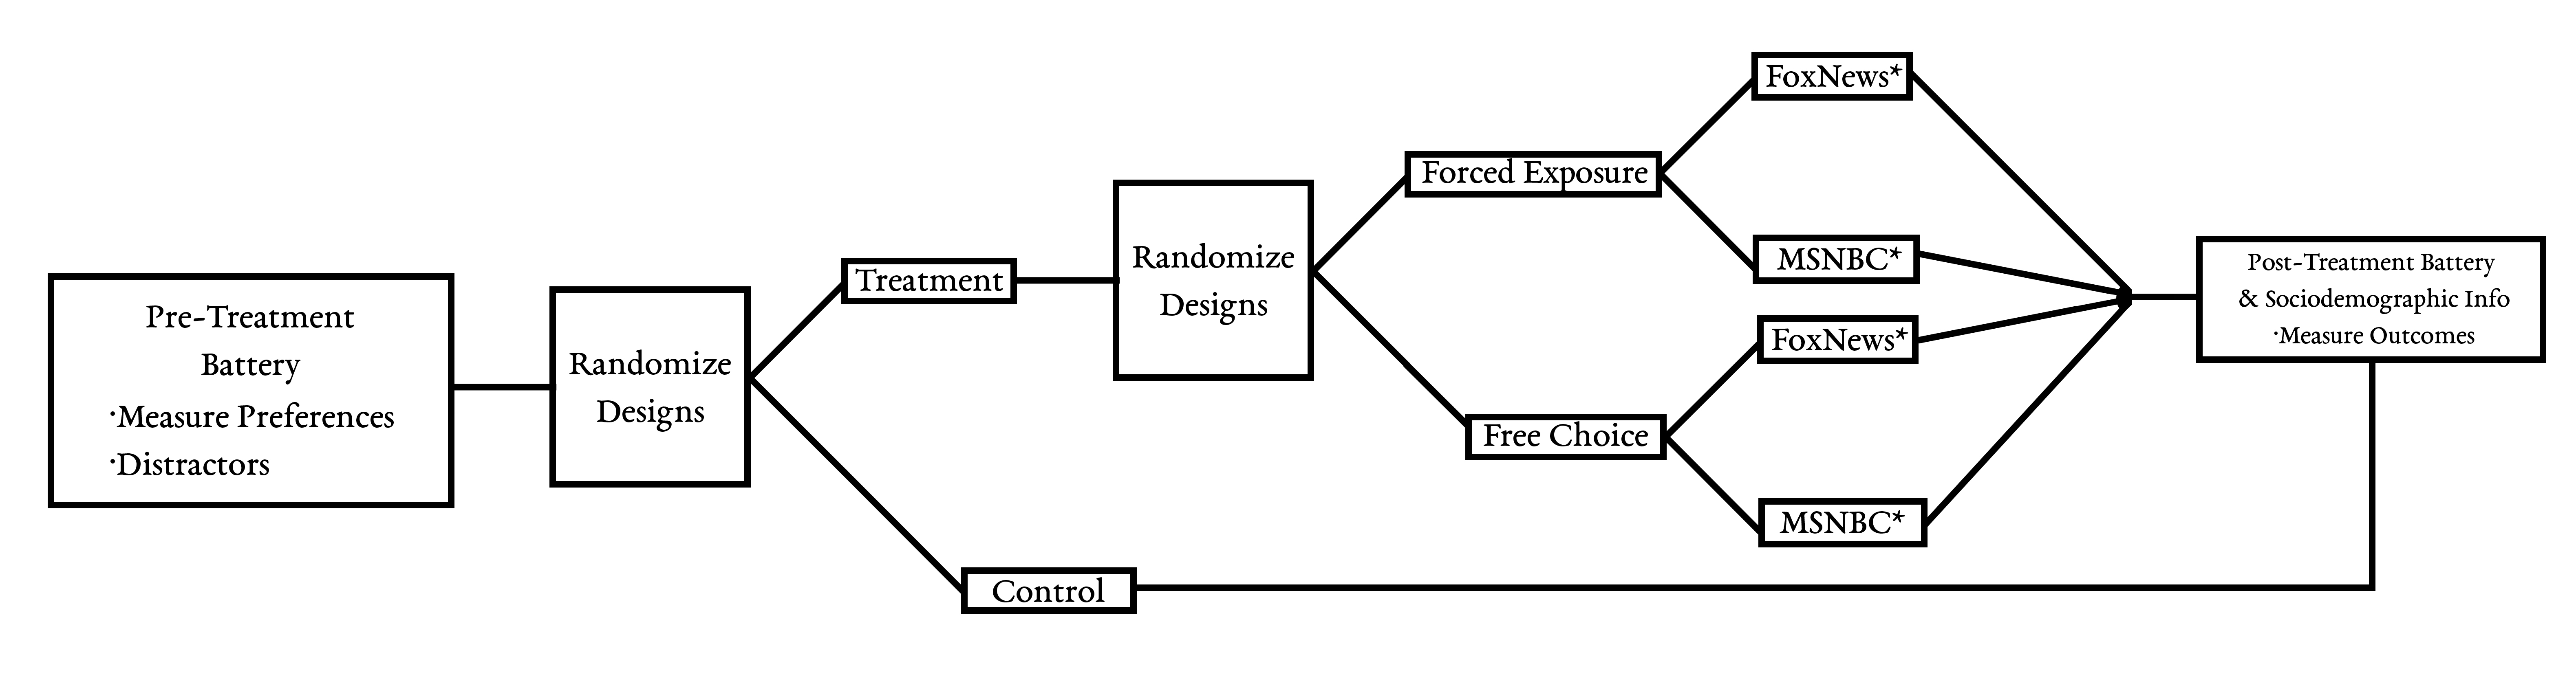
\includegraphics{Lab-Graphic.jpg}
\caption{Survey Flow}
\end{figure}

\hypertarget{outcome-measures}{%
\subsection{Outcome measures}\label{outcome-measures}}

We consider several outcome measures to capture immigration attitudes
and how the news story is received by participants. This section briefly
describes each outcome and outlines relevant items in the questionnaire
(see also full question wording at the end of the pre-analysis plan).
Unless otherwise specified, outcomes that are measured using multiple
variables will be combined in a additive scale. We are going to ensure
that all items load properly on a single factor and exclude those that
do not. Furthermore, we will report results using individual items in
the appendix.

\textbf{Economic impact of immigration:} Our first outcome of interest
captures the perceived economic impact of legal immigration. The news
article includes specific information about the number of people in the
US who are employed by immigrant-owned businesses as well as the total
amount of sales revenue of immigrant-owned businesses. As part of the
survey, participants are asked two questions covering these issues and
our goal is to examine whether the news article is sufficient to correct
related factual misperceptions (i.e., increase the proportion of correct
responses on two questions covering this information). Two additional
questions (analyzed separately) capture respondents' beliefs about how
much immigrants contribute to society by paying taxes and creating jobs.
Here, the outcome of interest is whether participants think that on
balance, legal immigration has a more positive impact rather than
creating a financial burden for society as a whole.

\textbf{Attitudes towards immigration:} Our second outcome measure
focuses on people's attitudes towards legal immigration. Specifically,
we ask participants whether they think that the number of immigrants in
the US should be increased or decreased. This item allows us to assess
whether the news article not only corrects factual misperceptions but
additionally induces attitude change.

\textbf{Trust in news sources:} As an additional check, we also include
a battery of items measuring trust in different news sources including
FoxNews and MSNBC. Since the content of the news article is held
constant between both news organizations, we can examine how exposure to
an atypical news story (in this case published by FoxNews) impacts
people's perception of the source itself.

In addition to these main variables, we evaluate four additional
outcomes and conduct a simple manipulation check. Note that by the
nature of the experimental design, these items can only be measured in
the two treatment arms of the experiment and are not included in the
control group.

\textbf{Engagement with tweet:} As described above, the tweet shown to
participants consists of a link to a news article. While the link itself
is not active and participants are never explicitly asked to click on
it, we can examine whether participants nevertheless try access the
article. Whether they attempt to do so is used as an unobstrusive
measure of the degree to which participants are interested in further
engaging with the content voluntarily.

\textbf{Response latencies:} In order to further assess the extent to
which respondents are interested in the article and comply with the
instructions to read it carefully, we also measure the amount of time
that individuals spend viewing the tweet and reading the news story.

\textbf{Sharing the article:} After reading the article, participants
are asked to report their willingness to share it on social media,
discuss it with friends, or whether they would be likely to seek out
more information regarding the topic of the tweet and story.

\textbf{Evaluation of the article:} Our final outcome measure consists
of a basic evaluation of the article, asking participants to disclose if
they found the article fair or unfair, hostile or friendly, bad or good,
skewed or balanced, American or un-American, and accurate or inaccurate.

\textbf{Manipulation Check:} In order to assess whether the tweet and
news article were actually read by participants, we include a brief
manipulation check. Specifically, respondents are asked which news
organization published the story and what topic was covered by it.

\hypertarget{hypotheses}{%
\subsection{Hypotheses}\label{hypotheses}}

Previous research examining the effectiveness of corrective information
showed that it does not always lead to attitude change even if
misperceptions are reduced (Hopkins, Sides, and Citrin 2019,
@thompson2019might). However, others find that media exposure can
persuade people to change their attitudes under certain conditions
(e.g., De Benedictis-Kessner et al., n.d.). Our study explores how the
way people access corrective information influences the likelihood of
its success in reducing misperceptions. In general, we expect that those
who were able to choose a news agency are more likely to pick a source
similar to their usual media diet. Additionally, we expect those who
read a news story from a trusted news source (and who are able to pick
the news agency) are more inclined to evaluate the article positively
and change their attitudes in the direction of the news article.

\hypertarget{main-analysis}{%
\subsubsection{Main analysis}\label{main-analysis}}

For the main outcome measures described above (i.e., immigration
attitudes and perceived economic impact), our analysis begins with two
basic comparisons between each treatment group and the control group:

\begin{itemize}
\tightlist
\item
  \textbf{H1a} {[}control vs.~forced exposure{]}: Participants who are
  assigned to a random news organization update their beliefs and
  attitudes in the direction of the article .
\item
  \textbf{H1b} {[}control vs.~free choice{]}: Participants who are free
  to choose a news organization update their beliefs and attitudes in
  the direction of the article.
\end{itemize}

In the context of the outcomes described previously, updating beliefs
and attitudes in the direction of the article refers to a decrease in
factual misperceptions about the economic impact of legal immigration
and more positive attitudes towards legal immigration more generally. Of
course, our main interest is to assess whether corrective information is
more effective if people are allowed to choose their preferred
information source than if they are assiged to one. We therefore
hypothesize that the free choice condition leads to a stronger
attitude/belief change than the forced exposure condition:

\begin{itemize}
\tightlist
\item
  \textbf{H1c} {[}forced exposure vs.~free choice{]}: Participants who
  are given the opportunity to choose a news organization are more
  likely to update their beliefs and attitudes in the direction of the
  article than participants who are randomly assigned to a news
  organization.
\end{itemize}

Note that this last comparison (\emph{H1c}) can also be evaluated using
the additional outcome measures described above (trust in news sources,
engagement with tweet, response latencies, sharing the article,
evaluation of the article), which are not included in the control group.
For each of these outcomes, we expect that the ability to choose their
preferred information source will increase engagement with the article
and therefore lead to more positive evaluations. Here, we also plan to
explore conditional treatment effects based on pre-treatment measures of
people's political predispositions (stereotypes towards immigrants,
whether immigration is seen as a major issue, ideology, partisanship)
and we will further examine whether the differences in \emph{H1c} are
conditional on participants being exposed to a news source that is
congruent with their usual media diet. Any difference between the forced
exposure and free choice condition could theoretically be driven either
by the fact that participants in the free choice condition tend to
select news organizations they are more sympathetic towards, or by the
fact alone that they are able to choose a source (i.e., the selection
process itself makes the information more effective). In order to
distinguish both possibilities, we will conduct an additional test where
we isolate the effect of forced exposure vs.~free choice while holding
the underlying news organization constant. Specifically, we are planning
to compare both conditions within groups of individuals who were exposed
to a congruent as compared to an incongruent source (either by choice or
by random assignment). Additional analyses outlined below will allow us
to further assess how endogeneous media exposure impacts the
effectiveness of corrective information.

\hypertarget{determinants-of-media-choice}{%
\subsubsection{Determinants of media
choice}\label{determinants-of-media-choice}}

Beyond this main analysis comparing the free choice and forced exposure
conditions, we are going to confirm whether respondents indeed choose
information sources that are consistent with their ideological
predisposition and usual media diet. This part of the analysis therefore
only focuses on the free choice arm of the experiment. Participants are
expected to engage in a biased search process, seeking out information
that is likely to support their preconceptions and avoiding evidence
that undercuts their beliefs (see Taber and Lodge 2006). This leads to
the following set of hypotheses regarding endogenous information search:

\begin{itemize}
\tightlist
\item
  \textbf{H2a:} When free to choose a news organization, conservatives
  (liberals) are more likely to pick FoxNews (MSNBC) than vice versa.
\item
  \textbf{H2b:} When free to choose a news organization, Republicans
  (Democrats) are more likely to pick FoxNews (MSNBC) than vice versa.
\item
  \textbf{H2c:} When free to choose a news organization, participants
  who report viewing FoxNews (MSNBC) more regularly are more likely to
  pick FoxNews (MSNBC).
\end{itemize}

\hypertarget{effects-of-corrective-information-conditional-on-preferred-media-choice}{%
\subsubsection{Effects of corrective information conditional on
preferred media
choice}\label{effects-of-corrective-information-conditional-on-preferred-media-choice}}

Lastly, we plan to examine whether there are systematic differences in
the effectiveness of corrective information by news sources themselves
(i.e., FoxNews vs.~MSNBC). The pre-treatment section of the
questionnaire includes items on respondents' usual media diet and
political predispositions. Respondents should be more inclined to update
their attitudes and beliefs if the article is published by a news
organization that is usually consistent with their priors:

\begin{itemize}
\tightlist
\item
  \textbf{H3a:} Conservatives (liberals) update their beliefs and
  attitudes more if they are randomly assigned to FoxNews (MSNBC).
\item
  \textbf{H3b:} Republicans (Democrats) update their beliefs and
  attitudes more if they are randomly assigned to FoxNews (MSNBC).
\item
  \textbf{H3c}: Participants who were randomly assigned to a news
  organization that is part of their regular media diet update their
  beliefs more than those who were assigned to a different news
  organization.
\end{itemize}

As a first step, these comparisons exclude the free choice arm of the
experiment and estimate treatment effects based on the randomly assigned
news organizations alone. Additionally, we are going to explore the
average choice-specific treatment effect (ACTE) following Knox et al.
(2019) to quantify the effect of corrective information conditional on
endogeneous media search (\emph{H3c}). This quantity of interest
captures the conditional average treatment effect for the subset of
participants who would choose a particular treatment option (i.e., the
effect of the article among those who would have chosen FoxNews or MSNBC
voluntarily).

\hypertarget{estimation-strategy}{%
\section{Estimation strategy}\label{estimation-strategy}}

\hypertarget{statistical-significance}{%
\subsection{Statistical significance}\label{statistical-significance}}

Throughout this study, we will use two-sided tests with an
\(\alpha\)-value of 0.05 as the cutoff for statistical significance. In
our graphical displays we will additionally plot 90\% intervals to
signal statistical significance at \(p<0.10\).

\hypertarget{missing-data}{%
\subsection{Missing data}\label{missing-data}}

Respondents who report ``don't know'' on the outcome measures (if
applicable) or who skipped the question will be treated as missing and
excluded from the respective analysis (basic listwise deletion). While
we are going to use the manipulation checks to evaluate whether
respondents read the information provided to them, we decided not to
drop respondents who failed to pass the manipulation checks in the
subsequent analyses (see for example Aronow, Baron, and Pinson 2018).

\hypertarget{main-analyses}{%
\subsection{Main analyses}\label{main-analyses}}

To test our hypotheses, we will rely on simple differences-in-means and
OLS estimators to compare the outcome measures between each treatment
and the control group, respectively. The main analyses will focus on the
average treatment effects relative to the control as well as the
difference between both treatment conditions themselves. The power
analyses reported below shows that given our sample size of 600, we have
85\% power to detect a 0.3 standard deviation effect between the
treatment and control group. Howver, we can only detect a 0.2 standard
deviation effect between both treatment conditions with 53\% power. We
will also consider heterogeneous treatment effects by pre-treatment
covariates (stereotypes towards immigrants, whether immigration is seen
as a major issue, and basic political predispositions) and we will
explore average choice-specific treatment effects (ACTE) following Knox
et al. (2019). Unfortunately, our power analysis below suggests that our
sample size is too small to reliably detect these conditional treatment
effects.

\hypertarget{power-analysis-basic-3-arm-design-ate-wo-differentiating-sources}{%
\subsubsection{Power analysis: basic 3-arm design (ATE w/o
differentiating
sources)}\label{power-analysis-basic-3-arm-design-ate-wo-differentiating-sources}}

\begin{Shaded}
\begin{Highlighting}[]
\NormalTok{N <{-}}\StringTok{ }\DecValTok{600}
\NormalTok{outcome\_means <{-}}\StringTok{ }\KeywordTok{c}\NormalTok{(}\DecValTok{0}\NormalTok{, }\FloatTok{.1}\NormalTok{, }\FloatTok{.3}\NormalTok{)}
\NormalTok{sd\_i <{-}}\StringTok{ }\DecValTok{1}

\NormalTok{population <{-}}\StringTok{ }\KeywordTok{declare\_population}\NormalTok{(}
  \DataTypeTok{N =}\NormalTok{ N, }\DataTypeTok{u =} \KeywordTok{rnorm}\NormalTok{(N, }\DataTypeTok{sd =}\NormalTok{ sd\_i))}

\NormalTok{potential\_outcomes <{-}}\StringTok{ }\KeywordTok{declare\_potential\_outcomes}\NormalTok{(}
  \DataTypeTok{formula =}\NormalTok{ Y }\OperatorTok{\textasciitilde{}}\StringTok{ }\NormalTok{outcome\_means[}\DecValTok{1}\NormalTok{] }\OperatorTok{*}\StringTok{ }\NormalTok{(Z }\OperatorTok{==}\StringTok{ "0"}\NormalTok{) }\OperatorTok{+}
\StringTok{    }\NormalTok{outcome\_means[}\DecValTok{2}\NormalTok{] }\OperatorTok{*}\StringTok{ }\NormalTok{(Z }\OperatorTok{==}\StringTok{ "1"}\NormalTok{) }\OperatorTok{+}
\StringTok{    }\NormalTok{outcome\_means[}\DecValTok{3}\NormalTok{] }\OperatorTok{*}\StringTok{ }\NormalTok{(Z }\OperatorTok{==}\StringTok{ "2"}\NormalTok{) }\OperatorTok{+}\StringTok{ }\NormalTok{u,}
  \DataTypeTok{conditions =} \KeywordTok{c}\NormalTok{(}\StringTok{"0"}\NormalTok{, }\StringTok{"1"}\NormalTok{, }\StringTok{"2"}\NormalTok{),}
  \DataTypeTok{assignment\_variables =}\NormalTok{ Z)}

\NormalTok{estimand <{-}}\StringTok{ }\KeywordTok{declare\_estimands}\NormalTok{(}
  \DataTypeTok{ate\_Y\_1\_0 =} \KeywordTok{mean}\NormalTok{(Y\_Z\_}\DecValTok{1} \OperatorTok{{-}}\StringTok{ }\NormalTok{Y\_Z\_}\DecValTok{0}\NormalTok{),}
  \DataTypeTok{ate\_Y\_2\_0 =} \KeywordTok{mean}\NormalTok{(Y\_Z\_}\DecValTok{2} \OperatorTok{{-}}\StringTok{ }\NormalTok{Y\_Z\_}\DecValTok{0}\NormalTok{),}
  \DataTypeTok{ate\_Y\_2\_1 =} \KeywordTok{mean}\NormalTok{(Y\_Z\_}\DecValTok{2} \OperatorTok{{-}}\StringTok{ }\NormalTok{Y\_Z\_}\DecValTok{1}\NormalTok{))}

\NormalTok{assignment <{-}}\StringTok{ }\KeywordTok{declare\_assignment}\NormalTok{(}
  \DataTypeTok{num\_arms =} \DecValTok{3}\NormalTok{,}
  \DataTypeTok{conditions =} \KeywordTok{c}\NormalTok{(}\StringTok{"0"}\NormalTok{, }\StringTok{"1"}\NormalTok{, }\StringTok{"2"}\NormalTok{),}
  \DataTypeTok{assignment\_variable =}\NormalTok{ Z)}

\NormalTok{reveal\_Y <{-}}\StringTok{ }\KeywordTok{declare\_reveal}\NormalTok{(}
  \DataTypeTok{assignment\_variables =}\NormalTok{ Z)}

\NormalTok{estimator <{-}}\StringTok{ }\KeywordTok{declare\_estimator}\NormalTok{(}
  \DataTypeTok{handler =} \ControlFlowTok{function}\NormalTok{(data) \{}
\NormalTok{    estimates <{-}}\StringTok{ }\KeywordTok{rbind.data.frame}\NormalTok{(}
      \DataTypeTok{ate\_Y\_1\_0 =} \KeywordTok{difference\_in\_means}\NormalTok{(}\DataTypeTok{formula =}\NormalTok{ Y }\OperatorTok{\textasciitilde{}}\StringTok{ }\NormalTok{Z, }\DataTypeTok{data =}\NormalTok{ data, }
                                      \DataTypeTok{condition1 =} \StringTok{"0"}\NormalTok{, }\DataTypeTok{condition2 =} \StringTok{"1"}\NormalTok{),}
      \DataTypeTok{ate\_Y\_2\_0 =} \KeywordTok{difference\_in\_means}\NormalTok{(}\DataTypeTok{formula =}\NormalTok{ Y }\OperatorTok{\textasciitilde{}}\StringTok{ }\NormalTok{Z, }\DataTypeTok{data =}\NormalTok{ data, }
                                      \DataTypeTok{condition1 =} \StringTok{"0"}\NormalTok{, }\DataTypeTok{condition2 =} \StringTok{"2"}\NormalTok{),}
      \DataTypeTok{ate\_Y\_2\_1 =} \KeywordTok{difference\_in\_means}\NormalTok{(}\DataTypeTok{formula =}\NormalTok{ Y }\OperatorTok{\textasciitilde{}}\StringTok{ }\NormalTok{Z, }\DataTypeTok{data =}\NormalTok{ data, }
                                      \DataTypeTok{condition1 =} \StringTok{"1"}\NormalTok{, }\DataTypeTok{condition2 =} \StringTok{"2"}\NormalTok{))}
    \KeywordTok{names}\NormalTok{(estimates)[}\KeywordTok{names}\NormalTok{(estimates) }\OperatorTok{==}\StringTok{ "N"}\NormalTok{] <{-}}\StringTok{ "N\_DIM"}
\NormalTok{    estimates}\OperatorTok{$}\NormalTok{estimator\_label <{-}}\StringTok{ }\KeywordTok{c}\NormalTok{(}\StringTok{"DIM (Z\_1 {-} Z\_0)"}\NormalTok{, }\StringTok{"DIM (Z\_2 {-} Z\_0)"}\NormalTok{,}
                                   \StringTok{"DID (Z\_2 {-} Z\_1)"}\NormalTok{)}
\NormalTok{    estimates}\OperatorTok{$}\NormalTok{estimand\_label <{-}}\StringTok{ }\KeywordTok{rownames}\NormalTok{(estimates)}
\NormalTok{    estimates}\OperatorTok{$}\NormalTok{estimate <{-}}\StringTok{ }\NormalTok{estimates}\OperatorTok{$}\NormalTok{coefficients}
\NormalTok{    estimates}\OperatorTok{$}\NormalTok{term <{-}}\StringTok{ }\OtherTok{NULL}
    \KeywordTok{return}\NormalTok{(estimates)}
\NormalTok{  \})}

\NormalTok{multi\_arm\_design <{-}}\StringTok{ }\NormalTok{population }\OperatorTok{+}\StringTok{ }\NormalTok{potential\_outcomes }\OperatorTok{+}\StringTok{ }
\StringTok{  }\NormalTok{assignment }\OperatorTok{+}\StringTok{ }\NormalTok{reveal\_Y }\OperatorTok{+}\StringTok{ }\NormalTok{estimand }\OperatorTok{+}\StringTok{ }\NormalTok{estimator}

\CommentTok{\# diagnose design based on 500 simulations}
\KeywordTok{diagnose\_design}\NormalTok{(multi\_arm\_design, }\DataTypeTok{diagnosands =} \KeywordTok{declare\_diagnosands}\NormalTok{(}
  \DataTypeTok{select =} \KeywordTok{c}\NormalTok{(}\StringTok{"power"}\NormalTok{, }\StringTok{"bias"}\NormalTok{)))}
\end{Highlighting}
\end{Shaded}

\begin{verbatim}
## 
## Research design diagnosis based on 500 simulations. Diagnosand estimates with bootstrapped standard errors in parentheses (100 replicates).
## 
##      Design Label Estimand Label Estimator Label N Sims  Power   Bias
##  multi_arm_design      ate_Y_1_0 DIM (Z_1 - Z_0)    500   0.16   0.00
##                                                         (0.02) (0.00)
##  multi_arm_design      ate_Y_2_0 DIM (Z_2 - Z_0)    500   0.87   0.00
##                                                         (0.01) (0.00)
##  multi_arm_design      ate_Y_2_1 DID (Z_2 - Z_1)    500   0.53   0.00
##                                                         (0.02) (0.00)
\end{verbatim}

\hypertarget{power-analysis-conditional-effects-depending-on-media-preference-acte-following-knox}{%
\subsubsection{Power analysis: conditional effects depending on media
preference (ACTE following
Knox)}\label{power-analysis-conditional-effects-depending-on-media-preference-acte-following-knox}}

\begin{Shaded}
\begin{Highlighting}[]
\NormalTok{Nforced <{-}}\StringTok{ }\KeywordTok{round}\NormalTok{(N}\OperatorTok{/}\DecValTok{3}\NormalTok{)}
\NormalTok{Sfox\_Afox <{-}}\StringTok{ }\FloatTok{.2} \CommentTok{\# note: S = preferred treatment, A = actual treatment}
\NormalTok{Sfox\_Amsnbc <{-}}\StringTok{ }\FloatTok{.0}
\NormalTok{Smsnbc\_Afox <{-}}\StringTok{ }\FloatTok{.3}
\NormalTok{Smsnbc\_Amsnbc <{-}}\StringTok{ }\FloatTok{.4}
\NormalTok{sd\_i <{-}}\StringTok{ }\DecValTok{1}

\NormalTok{population <{-}}\StringTok{ }\KeywordTok{declare\_population}\NormalTok{(}
  \DataTypeTok{N =}\NormalTok{ Nforced, }\DataTypeTok{u =} \KeywordTok{rnorm}\NormalTok{(Nforced, }\DataTypeTok{sd =}\NormalTok{ sd\_i))}

\NormalTok{potential\_outcomes <{-}}\StringTok{ }\KeywordTok{declare\_potential\_outcomes}\NormalTok{(}
  \DataTypeTok{formula =}\NormalTok{ Y }\OperatorTok{\textasciitilde{}}\StringTok{ }\DecValTok{0} \OperatorTok{+}
\StringTok{    }\NormalTok{Sfox\_Afox }\OperatorTok{*}\StringTok{ }\NormalTok{(Z }\OperatorTok{==}\StringTok{ "1"}\NormalTok{) }\OperatorTok{+}
\StringTok{    }\NormalTok{Sfox\_Amsnbc }\OperatorTok{*}\StringTok{ }\NormalTok{(Z }\OperatorTok{==}\StringTok{ "2"}\NormalTok{) }\OperatorTok{+}
\StringTok{    }\NormalTok{Smsnbc\_Afox }\OperatorTok{*}\StringTok{ }\NormalTok{(Z }\OperatorTok{==}\StringTok{ "3"}\NormalTok{) }\OperatorTok{+}
\StringTok{    }\NormalTok{Smsnbc\_Amsnbc }\OperatorTok{*}\StringTok{ }\NormalTok{(Z }\OperatorTok{==}\StringTok{ "4"}\NormalTok{) }\OperatorTok{+}\StringTok{ }\NormalTok{u,}
  \DataTypeTok{conditions =} \KeywordTok{c}\NormalTok{(}\StringTok{"1"}\NormalTok{, }\StringTok{"2"}\NormalTok{, }\StringTok{"3"}\NormalTok{,}\StringTok{"4"}\NormalTok{),}
  \DataTypeTok{assignment\_variables =}\NormalTok{ Z)}

\NormalTok{estimand <{-}}\StringTok{ }\KeywordTok{declare\_estimands}\NormalTok{(}
  \DataTypeTok{acte\_Y\_fox =} \KeywordTok{mean}\NormalTok{(Y\_Z\_}\DecValTok{1} \OperatorTok{{-}}\StringTok{ }\NormalTok{Y\_Z\_}\DecValTok{2}\NormalTok{),}
  \DataTypeTok{acte\_Y\_msnbc =} \KeywordTok{mean}\NormalTok{(Y\_Z\_}\DecValTok{4} \OperatorTok{{-}}\StringTok{ }\NormalTok{Y\_Z\_}\DecValTok{3}\NormalTok{))}

\NormalTok{assignment <{-}}\StringTok{ }\KeywordTok{declare\_assignment}\NormalTok{(}
  \DataTypeTok{num\_arms =} \DecValTok{4}\NormalTok{,}
  \DataTypeTok{conditions =} \KeywordTok{c}\NormalTok{(}\StringTok{"1"}\NormalTok{, }\StringTok{"2"}\NormalTok{, }\StringTok{"3"}\NormalTok{, }\StringTok{"4"}\NormalTok{),}
  \DataTypeTok{assignment\_variable =}\NormalTok{ Z)}

\NormalTok{reveal\_Y <{-}}\StringTok{ }\KeywordTok{declare\_reveal}\NormalTok{(}
  \DataTypeTok{assignment\_variables =}\NormalTok{ Z)}

\NormalTok{estimator <{-}}\StringTok{ }\KeywordTok{declare\_estimator}\NormalTok{(}
  \DataTypeTok{handler =} \ControlFlowTok{function}\NormalTok{(data) \{}
\NormalTok{    estimates <{-}}\StringTok{ }\KeywordTok{rbind.data.frame}\NormalTok{(}
      \DataTypeTok{acte\_Y\_fox =} \KeywordTok{difference\_in\_means}\NormalTok{(}\DataTypeTok{formula =}\NormalTok{ Y }\OperatorTok{\textasciitilde{}}\StringTok{ }\NormalTok{Z, }\DataTypeTok{data =}\NormalTok{ data, }
                                       \DataTypeTok{condition1 =} \StringTok{"2"}\NormalTok{, }\DataTypeTok{condition2 =} \StringTok{"1"}\NormalTok{),}
      \DataTypeTok{acte\_Y\_msnbc =} \KeywordTok{difference\_in\_means}\NormalTok{(}\DataTypeTok{formula =}\NormalTok{ Y }\OperatorTok{\textasciitilde{}}\StringTok{ }\NormalTok{Z, }\DataTypeTok{data =}\NormalTok{ data, }
                                         \DataTypeTok{condition1 =} \StringTok{"3"}\NormalTok{, }\DataTypeTok{condition2 =} \StringTok{"4"}\NormalTok{))}
    \KeywordTok{names}\NormalTok{(estimates)[}\KeywordTok{names}\NormalTok{(estimates) }\OperatorTok{==}\StringTok{ "N"}\NormalTok{] <{-}}\StringTok{ "N\_DIM"}
\NormalTok{    estimates}\OperatorTok{$}\NormalTok{estimator\_label <{-}}\StringTok{ }\KeywordTok{c}\NormalTok{(}\StringTok{"DIM (Z\_1 {-} Z\_2)"}\NormalTok{, }\StringTok{"DIM (Z\_4 {-} Z\_3)"}\NormalTok{)}
\NormalTok{    estimates}\OperatorTok{$}\NormalTok{estimand\_label <{-}}\StringTok{ }\KeywordTok{rownames}\NormalTok{(estimates)}
\NormalTok{    estimates}\OperatorTok{$}\NormalTok{estimate <{-}}\StringTok{ }\NormalTok{estimates}\OperatorTok{$}\NormalTok{coefficients}
\NormalTok{    estimates}\OperatorTok{$}\NormalTok{term <{-}}\StringTok{ }\OtherTok{NULL}
    \KeywordTok{return}\NormalTok{(estimates)}
\NormalTok{  \})}

\NormalTok{multi\_arm\_design <{-}}\StringTok{ }\NormalTok{population }\OperatorTok{+}\StringTok{ }\NormalTok{potential\_outcomes }\OperatorTok{+}\StringTok{ }
\StringTok{  }\NormalTok{assignment }\OperatorTok{+}\StringTok{ }\NormalTok{reveal\_Y }\OperatorTok{+}\StringTok{ }\NormalTok{estimand }\OperatorTok{+}\StringTok{ }\NormalTok{estimator}

\CommentTok{\# diagnose design based on 500 simulations}
\KeywordTok{diagnose\_design}\NormalTok{(multi\_arm\_design, }\DataTypeTok{diagnosands =} \KeywordTok{declare\_diagnosands}\NormalTok{(}
  \DataTypeTok{select =} \KeywordTok{c}\NormalTok{(}\StringTok{"power"}\NormalTok{, }\StringTok{"bias"}\NormalTok{)))}
\end{Highlighting}
\end{Shaded}

\begin{verbatim}
## 
## Research design diagnosis based on 500 simulations. Diagnosand estimates with bootstrapped standard errors in parentheses (100 replicates).
## 
##      Design Label Estimand Label Estimator Label N Sims  Power   Bias
##  multi_arm_design     acte_Y_fox DIM (Z_1 - Z_2)    500   0.19  -0.00
##                                                         (0.02) (0.01)
##  multi_arm_design   acte_Y_msnbc DIM (Z_4 - Z_3)    500   0.09   0.00
##                                                         (0.01) (0.01)
\end{verbatim}

\hypertarget{full-questionnaire}{%
\section{Full Questionnaire}\label{full-questionnaire}}

\hypertarget{survey-flow-overview}{%
\subsection{Survey Flow Overview}\label{survey-flow-overview}}

\begin{itemize}
\tightlist
\item
  Pre-treatment measures:

  \begin{itemize}
  \tightlist
  \item
    Media usage
  \item
    Stereotype battery
  \item
    Political attitudes \& participation
  \end{itemize}
\item
  Experimental manipulation:

  \begin{itemize}
  \tightlist
  \item
    Tweets
  \item
    Full story
  \item
    Attention checks \& article evaluation
  \end{itemize}
\item
  Post-treatment measures:

  \begin{itemize}
  \tightlist
  \item
    Attitudes towards immigration
  \item
    Trust in news sources
  \item
    Sociodemographics
  \end{itemize}
\end{itemize}

\hypertarget{pre-treatment-measures}{%
\subsection{Pre-treatment measures}\label{pre-treatment-measures}}

\hypertarget{block-1-media-usage}{%
\subsubsection{Block 1: Media usage}\label{block-1-media-usage}}

First, we want to ask a few questions about your current media diet.

\textbf{{[}smedia{]}} \emph{(show same response options for each,
randomize order)} On average, how often do you use the following social
media platforms?

\begin{itemize}
\tightlist
\item
  YouTube
\item
  Facebook
\item
  Instagram
\item
  Twitter
\item
  Tumblr
\end{itemize}

\begin{enumerate}
\def\labelenumi{\arabic{enumi}.}
\tightlist
\item
  Several times a day
\item
  About once a day
\item
  3 to 6 days a week
\item
  1 to 2 days a week
\item
  Every few weeks
\item
  Less often
\item
  Never
\item
  Don't Know
\end{enumerate}

\textbf{{[}tv{]}} \emph{(show same response options for each, randomize
order)} On average, how often do you watch \emph{political} news on the
following TV channels (including online content)?

\begin{itemize}
\tightlist
\item
  Fox News
\item
  MSNBC
\item
  CNN
\item
  NBC
\item
  CBS
\end{itemize}

\begin{enumerate}
\def\labelenumi{\arabic{enumi}.}
\tightlist
\item
  Several times a day
\item
  About once a day
\item
  3 to 6 days a week
\item
  1 to 2 days a week
\item
  Every few weeks
\item
  Less often
\item
  Never
\item
  Don't Know
\end{enumerate}

\textbf{{[}print{]}} \emph{(show same response options for each,
randomize order)} And how often do you read about articles about
\emph{politics} in the following newspapers (online or offline)?

\begin{itemize}
\tightlist
\item
  New York Times
\item
  Washington Post
\item
  Wall Street Journal
\item
  USA Today
\item
  New York Post
\end{itemize}

\begin{enumerate}
\def\labelenumi{\arabic{enumi}.}
\tightlist
\item
  Several times a day
\item
  About once a day
\item
  3 to 6 days a week
\item
  1 to 2 days a week
\item
  Every few weeks
\item
  Less often
\item
  Never
\item
  Don't Know
\end{enumerate}

\hypertarget{block-2-stereotype-battery}{%
\subsubsection{Block 2: Stereotype
battery}\label{block-2-stereotype-battery}}

Next are some questions about different groups in our society.

\textbf{{[}st\_job{]}} \emph{(show same response options for each,
randomize order)} Do you think that people in the following groups tend
to be ``intelligent'' or ``unintelligent''?

\begin{itemize}
\tightlist
\item
  Farmers
\item
  Teachers
\item
  Lawyers
\item
  Politicians
\end{itemize}

\begin{enumerate}
\def\labelenumi{(\arabic{enumi})}
\tightlist
\item
  Intelligent - (7) Unintelligent, (8) DK
\end{enumerate}

\textbf{{[}st\_race{]}} \emph{(show same response options for each,
randomize order)} And do you think that people in the following groups
are ``hard-working'' or ``lazy''?

\begin{itemize}
\tightlist
\item
  Whites
\item
  Blacks
\item
  Hispanic-Americans
\item
  Asian-Americans
\end{itemize}

\begin{enumerate}
\def\labelenumi{(\arabic{enumi})}
\tightlist
\item
  Hard-working - (7) Lazy, (8) DK
\end{enumerate}

\textbf{{[}st\_age{]}} \emph{(show same response options for each)} And
do you think that people in the following groups are ``generous'' or
``selfish''?

\begin{itemize}
\tightlist
\item
  Silent Generation (born 1945 and before)
\item
  Baby Boomers (born 1946-1964)
\item
  Generation X (born 1965-1976)
\item
  Millennials (born 1977-1995)
\end{itemize}

\begin{enumerate}
\def\labelenumi{(\arabic{enumi})}
\tightlist
\item
  Generous - (7) Selfish, (8) DK
\end{enumerate}

\hypertarget{block-3-political-attitudes-participation}{%
\subsubsection{Block 3: Political attitudes \&
participation}\label{block-3-political-attitudes-participation}}

Next, we would like you to answer a few questions about your political
viewpoints.

\textbf{{[}polint{]}} How often do you pay attention to what's going on
in government and politics?

\begin{enumerate}
\def\labelenumi{\arabic{enumi}.}
\tightlist
\item
  Always
\item
  Most of the time
\item
  Sometimes
\item
  Hardly at all
\item
  Never
\end{enumerate}

\textbf{{[}problem{]}} \emph{(randomize order)}
What~do~you~think~are~the~most~important~problems~facing~this~country?~Please
rank the following issues from the most important to the least
important.

\begin{enumerate}
\def\labelenumi{\arabic{enumi}.}
\tightlist
\item
  Economy
\item
  Terrorism
\item
  Immigration
\item
  Health Care
\item
  Environment
\end{enumerate}

\textbf{{[}ideol{]}} Thinking about politics these days, how would you
describe your own political viewpoint?

\begin{enumerate}
\def\labelenumi{\arabic{enumi}.}
\tightlist
\item
  Very liberal
\item
  Liberal
\item
  Slightly liberal
\item
  Moderate
\item
  Slightly conservative
\item
  Conservative
\item
  Very conservative
\item
  Not sure
\end{enumerate}

\textbf{{[}pid{]}} Generally speaking, do you think of yourself as a
Republican, a Democrat, an independent, or other?

\begin{enumerate}
\def\labelenumi{\arabic{enumi}.}
\tightlist
\item
  Republican
\item
  Democrat
\item
  Independent
\item
  Other
\end{enumerate}

\textbf{{[}pid\_lean{]}} \emph{(if {[}pid{]} == other \textbar{}
independent)} Do you think of yourself as CLOSER to the Republican party
or to the Democratic party?

\begin{enumerate}
\def\labelenumi{\arabic{enumi}.}
\tightlist
\item
  Republican party
\item
  Democratic party
\item
  Neither party
\end{enumerate}

\textbf{{[}pid\_rep/pid\_dem{]}} \emph{(if {[}pid{]} == Republican
\textbar{} Democrat)} Would you consider yourself a strong
Republican/Democrat or a not very strong Republican/Democrat?

\begin{enumerate}
\def\labelenumi{\arabic{enumi}.}
\tightlist
\item
  Strong
\item
  Not very strong
\end{enumerate}

\hypertarget{experimental-manipulation}{%
\subsection{Experimental manipulation}\label{experimental-manipulation}}

\hypertarget{instructions-for-participants}{%
\subsubsection{Instructions for
participants}\label{instructions-for-participants}}

\begin{itemize}
\tightlist
\item
  \textbf{If treatment condition = choice}

  \begin{itemize}
  \item
    In the following section, we are going to show you a random tweet
    drawn from the accounts of two large news organizations. You can
    choose from which Twitter account the random tweet will be drawn.
    Afterwards, we are going to ask you some questions about the content
    of the news story.
  \item
    \textbf{{[}choice{]}} \emph{(randomize order)} From which Twitter
    account would you like to view a random tweet?

    \begin{enumerate}
    \def\labelenumi{\arabic{enumi}.}
    \tightlist
    \item
      Fox News
    \item
      MSNBC
    \end{enumerate}
  \end{itemize}
\item
  \textbf{If treatment condition = assigned}

  \begin{itemize}
  \item
    In the following section, we are going to show you a random tweet
    drawn from the accounts of several large news organizations.
    Afterwards, we are going to ask you some questions about the content
    of the news story.
  \item
    \textbf{{[}assigned{]}} \emph{(assignment to account invisible to
    participant)}

    \begin{enumerate}
    \def\labelenumi{\arabic{enumi}.}
    \tightlist
    \item
      Fox News
    \item
      MSNBC
    \end{enumerate}
  \end{itemize}
\end{itemize}

\hypertarget{tweets}{%
\subsubsection{Tweets}\label{tweets}}

\begin{figure}
\centering

\includegraphics[width=0.5\textwidth,height=\textheight]{../material/tweets/fox_popular.png}
\caption{Fox News}
\end{figure}

\begin{figure}
\centering

\includegraphics[width=0.5\textwidth,height=\textheight]{../material/tweets/msnbc_popular.png}
\caption{MSNBC}
\end{figure}

\hypertarget{introduction-for-full-story}{%
\subsubsection{Introduction for full
story}\label{introduction-for-full-story}}

Next, we will show you the content of the article linked in the previous
tweet. \textbf{Please read the story carefully.} Keep in mind that we
will ask you questions about the content of the article afterwards.

\emph{There will be a brief pause on the next screen so you can read the
story.} At the end of the pause, an arrow will appear at the bottom of
the screen. Once the arrow appears, you may move on to the next screen
of the survey by clicking on the arrow.

\hypertarget{full-story-immigrant-owned-businesses-on-the-rise}{%
\subsubsection{Full Story: Immigrant-owned Businesses on the
Rise}\label{full-story-immigrant-owned-businesses-on-the-rise}}

William Hall \textbar{} {[}Fox News/MSNBC{]}

A recent report released using U.S. Census Bureau data states that
immigrant-owned businesses employed over 8 million workers in fiscal
year 2019, up from 2018 totals. These businesses also experienced an
increase in the total amount of sales revenue, which rose to almost
\$1.3 trillion during the same period.

These statistics are borne out of hundreds of success stories across
many different sectors of the economy, especially the service industry.

\begin{figure}
\centering
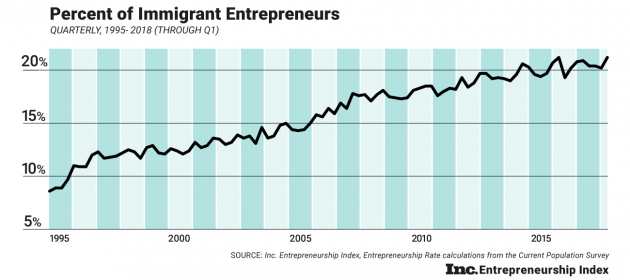
\includegraphics[width=0.45\textwidth,height=\textheight]{../material/fig/immig_entrepreneurs.png}
\caption{Percent of Immigrant Entrepreneurs}
\end{figure}

Eduardo Rodriguez, a 62 year old immigrant living in the Little Village
neighborhood of Chicago, is a perfect example of this success. In an
area of the city that has an unemployment rate of 13 percent and an
annual median income of \$30,000--less than half of the national
average--the Little Village community faces considerable economic
challenges. However, these conditions have not stopped Rodriguez. He
currently owns and operates four Dulcelandia stores in Little Village,
each one packed with over 1,000 types of delicious candies from his home
country of Mexico.

After immigrating here in 1966, Rodriguez opened his first store and it
became an instant gathering spot in the neighborhood. ``People seem to
really like what we are doing, and I'm grateful that I had the
opportunity to do this in the United States. It takes a lot of work and
sacrifice -- we're fulfilling a niche market that people really want to
buy from.''

Following in her father's footsteps, Rodriguez's daughter, Eve Rodriguez
Montoya, has also opened up a handful of shops that specialize in
healthy frozen yogurts with some Mexican-inspired flavors.

``Our community is very strong and hard-working -- resilient and
resourceful,'' she said. ``I'd say come to our community, get to know
our people. Shop at our locations and see for yourself -- Little Village
is full of people who came to this country to achieve the American
Dream.''

The Rodriguez's story is just one of many. As more immigrants look to
open their own businesses and employ more workers, many markets, both
broad and niche, will continue to expand and provide more fuel to an
already strong economy.

\emph{William Hall is a Business Reporter for {[}Fox News/MSNBC{]}.}

\hypertarget{attention-checks-article-evaluation}{%
\subsubsection{Attention checks \& article
evaluation}\label{attention-checks-article-evaluation}}

Please answer the following questions about the tweet as well as the
article you just read.

\textbf{{[}source{]}} \emph{(randomize order)} Which Twitter account /
news organization published the story?

\begin{enumerate}
\def\labelenumi{\arabic{enumi}.}
\tightlist
\item
  Fox News
\item
  MSNBC
\item
  New York Times
\item
  Wall Street Journal
\item
  Other
\item
  Don't know
\end{enumerate}

\textbf{{[}about{]}} \emph{(randomize order)} Broadly speaking, what was
the news story about?

\begin{enumerate}
\def\labelenumi{\arabic{enumi}.}
\tightlist
\item
  Immigrant-owned businesses
\item
  Stock market development
\item
  Innovation in the automotive industry
\item
  Young entrepreneurs in Silicon Valley
\item
  Don't know
\end{enumerate}

\textbf{{[}actions{]}} Thinking about the news article you just read,
how likely would you be to:

\begin{itemize}
\tightlist
\item
  Discuss the story with a friend
\item
  Forward the story to a friend or colleague via email
\item
  Post a link to the story on a social networking site, such as Facebook
  or Twitter
\item
  Seek out additional information from another source on the topic
  featured in the story
\end{itemize}

\begin{enumerate}
\def\labelenumi{(\arabic{enumi})}
\tightlist
\item
  Very likely - (4) Not likely, (7) Not sure
\end{enumerate}

\textbf{{[}wordpairs{]}} \emph{(randomize order)} Below, you will find a
list of pairs of words. Please rate the news article you just read on
each of the pairs of words.

\begin{itemize}
\tightlist
\item
  {[}fair{]} (1) Fair - (5) Unfair
\item
  {[}hostile{]} (1) Hostile - (5) Friendly
\item
  {[}bad{]} (1) Bad - (5) Good
\item
  {[}skewed{]} (1) Skewed - (5) balanced
\item
  {[}american{]} (1) American - (5) Un-American
\item
  {[}accurate{]} (1) Accurate - (5) Inaccurate
\end{itemize}

\hypertarget{post-treatment-measures}{%
\subsection{Post-treatment measures}\label{post-treatment-measures}}

\hypertarget{block-1-attitudes-towards-immigration}{%
\subsubsection{Block 1: Attitudes towards
immigration}\label{block-1-attitudes-towards-immigration}}

\emph{(only show this message in the control condition)} In this
section, we want to ask you a few questions about immigration.

\textbf{{[}employ{]}} Across the United States, how many workers --
immigrant and US-born -- do you think are employed by immigrant-owned
businesses?

\begin{enumerate}
\def\labelenumi{\arabic{enumi}.}
\tightlist
\item
  Less than 500,000
\item
  500,000 - 1 million
\item
  1 million - 5 million
\item
  5 million - 10 million
\item
  More than 10 million
\end{enumerate}

\textbf{{[}sales{]}} Taking your best guess, what was the total amount
of sales revenue of immigrant-owned businesses in the last year?

\begin{enumerate}
\def\labelenumi{\arabic{enumi}.}
\tightlist
\item
  Less than \$500 billion
\item
  \$500 billion - \$1 trillion
\item
  \$1 trillion - \$1.5 trillion
\item
  \$1.5 trillion - \$2 trillion
\item
  More than \$2 trillion
\end{enumerate}

\emph{(only show this message in the treatment conditions)} In this
section, we want to ask you a few questions about immigration in
general.

\textbf{{[}immig{]}} Do you think the number of immigrants from foreign
countries who are permitted to come to the United States to live should
be\ldots?

\begin{enumerate}
\def\labelenumi{\arabic{enumi}.}
\tightlist
\item
  Increased a lot
\item
  Increased a little
\item
  Left the same
\item
  Decreased a little
\item
  Decreased a lot
\end{enumerate}

\emph{(randomize order of remaining questions)}

\textbf{{[}taxes{]}} Most people who come to live in the U.S. work and
pay taxes. They also use health and social services. On balance, do you
think people who come here take out more than they put in or put in more
than they take out?

\begin{itemize}
\tightlist
\item
  0 (Generally take out more) - 10 (Generally put in more)
\end{itemize}

\textbf{{[}taxes\_oe{]}} Please explain your answer to the previous
question in a few short sentences.

\begin{itemize}
\tightlist
\item
  \emph{TEXTBOX}
\end{itemize}

\textbf{{[}jobs{]}} On average, would you say that people who come to
live here from other countries will take jobs away from people already
here or add to the economy by creating additional jobs?

\begin{itemize}
\tightlist
\item
  0 (Take jobs away) - 10 (Create additional jobs)
\end{itemize}

\textbf{{[}jobs\_oe{]}} Please explain your answer to the previous
question in a few short sentences.

\begin{itemize}
\tightlist
\item
  \emph{TEXTBOX}
\end{itemize}

\hypertarget{block-2-trust-in-news-sources}{%
\subsubsection{Block 2: Trust in news
sources}\label{block-2-trust-in-news-sources}}

Let's briefly return to the different media sources mentioned at the
beginning of the survey.

\textbf{{[}tv\_trust{]}} \emph{(show same response options for each,
randomize order)} Overall, how often can you trust the following TV
channels that their political news reporting is accurate?

\begin{itemize}
\tightlist
\item
  Fox News
\item
  MSNBC
\item
  CNN
\item
  NBC
\item
  CBS
\end{itemize}

\begin{enumerate}
\def\labelenumi{\arabic{enumi}.}
\tightlist
\item
  Always
\item
  Most of the time
\item
  About half the time
\item
  Sometimes
\item
  Never
\item
  Don't Know
\end{enumerate}

\textbf{{[}print\_trust{]}} \emph{(show same response options for each,
randomize order)} And how often can you trust the following newspapers
that their political reporting is accurate?

\begin{itemize}
\tightlist
\item
  New York Times
\item
  Washington Post
\item
  Wall Street Journal
\item
  USA Today
\item
  New York Post
\end{itemize}

\begin{enumerate}
\def\labelenumi{\arabic{enumi}.}
\tightlist
\item
  Always
\item
  Most of the time
\item
  About half the time
\item
  Sometimes
\item
  Never
\item
  Don't Know
\end{enumerate}

\hypertarget{block-3-sociodemographics}{%
\subsubsection{Block 3:
Sociodemographics}\label{block-3-sociodemographics}}

This almost completes our survey, we only need some additional
information about your background.

\textbf{{[}age{]}} What is your age?

\begin{itemize}
\tightlist
\item
  \emph{TEXTBOX}
\end{itemize}

\textbf{{[}gender{]}} Do you consider yourself Male, Female, or other?

\begin{enumerate}
\def\labelenumi{\arabic{enumi}.}
\tightlist
\item
  Male
\item
  Female
\item
  Other
\end{enumerate}

\textbf{{[}usborn{]}} Were you born in the United States?

\begin{enumerate}
\def\labelenumi{\arabic{enumi}.}
\tightlist
\item
  Yes
\item
  No
\end{enumerate}

\textbf{{[}usborn\_year{]}} \emph{(only ask if {[}usborn{]}==0)} When
did you first arrive to live in the US?

\begin{itemize}
\tightlist
\item
  \emph{TEXTBOX}
\end{itemize}

\textbf{{[}zip{]}} What is your zip code?

\begin{itemize}
\tightlist
\item
  \emph{TEXTBOX} \emph{(response not required)}
\end{itemize}

\textbf{{[}zip\_time{]}} \emph{(only ask if zip code is entered)} And
how long have you lived at your current zip code?

\begin{enumerate}
\def\labelenumi{\arabic{enumi}.}
\tightlist
\item
  Less than a year
\item
  1 to 3 years
\item
  3 to 5 years
\item
  More than 5 years
\item
  Don't Know
\end{enumerate}

\textbf{{[}race{]}} What racial or ethnic group best describes you?

\begin{enumerate}
\def\labelenumi{\arabic{enumi}.}
\tightlist
\item
  Asian/Pacific Islanders
\item
  Black or African-American (non-Hispanic)
\item
  Caucasian/White (non-Hispanic)
\item
  Hispanic or Latino
\item
  Middle eastern
\item
  Native American or Aleut
\item
  Other
\end{enumerate}

\textbf{{[}educ{]}} What is the highest level of education that you have
completed?

\begin{enumerate}
\def\labelenumi{\arabic{enumi}.}
\tightlist
\item
  Less than a high school diploma
\item
  Graduated high school or GED
\item
  Some college but no college degree
\item
  Graduated 2-year college
\item
  Graduated 4-year college
\item
  Completed post-graduate or professional school, with degree
\item
  Don't know
\end{enumerate}

\textbf{{[}income{]}} Thinking back over the last year, what was your
family's annual income?

\begin{enumerate}
\def\labelenumi{\arabic{enumi}.}
\tightlist
\item
  Less than \$20,000
\item
  \$20,000 - \$39,999
\item
  \$40,000 - \$59,999
\item
  \$60,000 - \$79,999
\item
  \$80,000 - \$99,999
\item
  \$100,000 - \$119,999
\item
  \$120,000 or more
\item
  Prefer not to say
\end{enumerate}

\textbf{{[}marital{]}} Which of the following best describes your
marital status?

\begin{enumerate}
\def\labelenumi{\arabic{enumi}.}
\tightlist
\item
  Single, never married
\item
  Married
\item
  Divorced
\item
  Separated
\item
  Widowed
\item
  Living with partner
\end{enumerate}

\textbf{{[}church{]}} Not counting weddings and funerals, how often do
you attend religious services?

\begin{enumerate}
\def\labelenumi{\arabic{enumi}.}
\tightlist
\item
  Never
\item
  Less than once a year
\item
  Once a year
\item
  Several times a year
\item
  Once a month
\item
  Two to three times a month
\item
  Nearly every week
\item
  Every week
\item
  More than once per week
\end{enumerate}

\textbf{{[}comments{]}} Thank you for answering our survey. Do you have
any comments for us?

\begin{itemize}
\tightlist
\item
  \emph{TEXTBOX}
\end{itemize}

\textbf{{[}debriefing{]}} \emph{(do not show in control condition)}
\emph{Note}: The news article you read was written specifically for the
purpose of this study. While the information provided in the article is
accurate, it was not originally published in this format. If you have
any questions or concerns, please contact the principal investigator
Dr.~Patrick Kraft
(\href{mailto:kraftp@uwm.edu}{\nolinkurl{kraftp@uwm.edu}}).

\hypertarget{references}{%
\section*{References}\label{references}}
\addcontentsline{toc}{section}{References}

\hypertarget{refs}{}
\begin{cslreferences}
\leavevmode\hypertarget{ref-aronow2018note}{}%
Aronow, Peter M, Jonathon Baron, and Lauren Pinson. 2018. ``A Note on
Dropping Experimental Subjects Who Fail a Manipulation Check.''
\emph{Political Analysis}, 1--18.

\leavevmode\hypertarget{ref-benedictis2019persuading}{}%
De Benedictis-Kessner, Justin, Matthew A Baum, Adam J Berinsky, and
Teppei Yamamoto. n.d. ``Persuading the Enemy: Estimating the Persuasive
Effects of Partisan Media with the Preference-Incorporating Choice and
Assignment Design.'' \emph{American Political Science Review}, 1--15.

\leavevmode\hypertarget{ref-hopkins2019muted}{}%
Hopkins, Daniel J, John Sides, and Jack Citrin. 2019. ``The Muted
Consequences of Correct Information About Immigration.'' \emph{The
Journal of Politics} 81 (1): 315--20.

\leavevmode\hypertarget{ref-kennedy2018shape}{}%
Kennedy, Ryan, Scott Clifford, Tyler Burleigh, Philip Waggoner, and Ryan
Jewell. 2018. ``The Shape of and Solutions to the Mturk Quality
Crisis.'' \emph{Available at SSRN}.

\leavevmode\hypertarget{ref-knox2019design}{}%
Knox, Dean, Teppei Yamamoto, Matthew A Baum, and Adam J Berinsky. 2019.
``Design, Identification, and Sensitivity Analysis for Patient
Preference Trials.'' \emph{Journal of the American Statistical
Association}, 1--27.

\leavevmode\hypertarget{ref-thompson2019might}{}%
Swire-Thompson, Briony, Ullrich K. H. Ecker, Stephan Lewandowsky, and
Adam J. Berinsky. 2019. ``They Might Be a Liar but They're My Liar:
Source Evaluation and the Prevalence of Misinformation.''
\emph{Political Psychology} forthcoming.
\url{https://doi.org/10.1111/pops.12586}.

\leavevmode\hypertarget{ref-Taber2006}{}%
Taber, Charles S., and Milton Lodge. 2006. ``Motivated Skepticism in the
Evaluation of Political Beliefs.'' \emph{American Journal of Political
Science} 50 (3): 755--69.
\url{https://doi.org/10.1111/j.1540-5907.2006.00214.x}.
\end{cslreferences}


\end{document}
